\chapter{Abläufe}

\section{Präprozessor}
\begin{figure}[H]
  \centering
  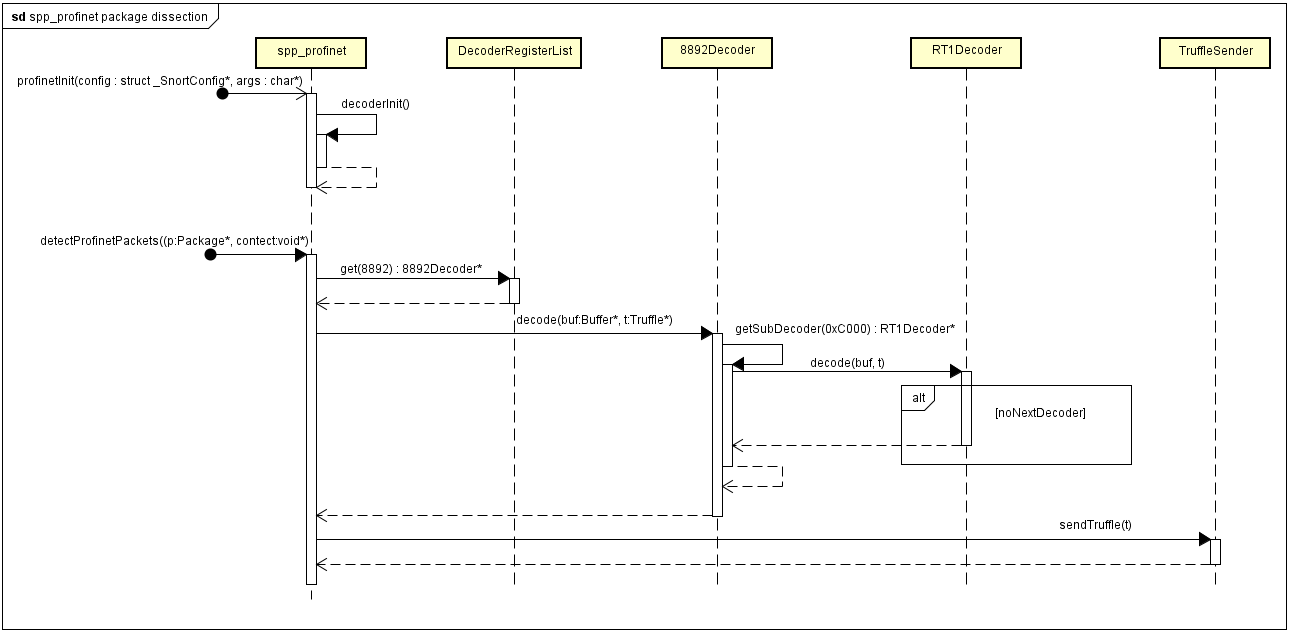
\includegraphics[width=\textwidth]{../diagramimages/spp-profinet-package-dissection.png}
  \caption[Sequenzdiagramm \gls{sppname} package dissection]{Sequenzdiagramm \gls{sppname} package dissection}
\end{figure}

In dieser Sequenz werden zwei zentrale Aufrufe von \gls{snort} im \gls{praeprozessor} \gls{sppname} dargestellt. Zum Einen im oberen Teil die Initialisierung des \gls{praeprozessor}s durch einen Init-Aufruf, sowie der \gls{praeprozessor}-interne Aufbau des DecoderRegisters. Dieser Registrierungsvorgang wurde im Diagramm aus Platzgründen eingespaart. Darin wird jeder als C-Datei vorhandene Decoder instanziiert und bei der DecoderRegisterList registriert. Dieser Vorgang legt die Grundlage für den Decoder-Baum-Ablauf, welcher exemplarisch als zweiter unterer Teil des Sequenzdiagramms modelliert wurde. Für jedes empfangene Paket ruft \gls{snort} die detectProfinetPackets in \sppname auf und übergibt eine Packetpointer. Basierend auf dem Ethertype wählt die DecoderRegisterList den ersten Decoder aus und übergibt den Pointer. \gls{sppname} ruft in diesem Decoder die decode-Methode auf, welche intern basierend auf gefundenen Informationen, sich einen seiner Subdecoder aussucht und in diesem die decode-Methode aufruft. Dieser rekursive Schritt wird solange wiederholt, bis kein Subdecoder mehr vorhanden ist oder das Ende des \gls{paket}s gefunden wurde.
Nach der Rückkehr der Methoden wird das fertige Truffle mit dem TruffleSender in Richtung \gls{programname} per \gls{ipc} verschickt.


\section{\gls{programname}}
\subsection{AddPacketDataCommand}
\begin{figure}[H]
  \centering
  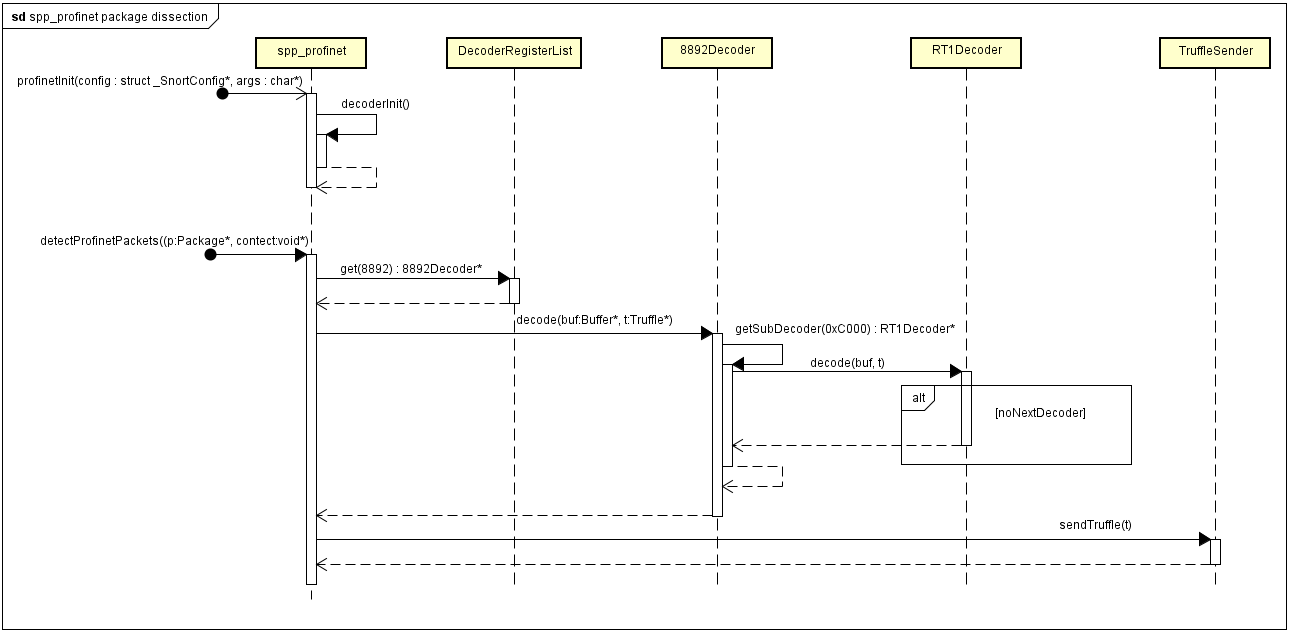
\includegraphics[width=\textwidth]{../diagramimages/spp-profinet-package-dissection.png}
  \caption[Sequenzdiagramm AddPacketData]{Sequenzdiagramm AddPacketData}
\end{figure}

Lorem ipsum dolor sit amet, consetetur sadipscing elitr, sed diam nonumy eirmod tempor invidunt ut labore et dolore magna aliquyam erat, sed diam voluptua. At vero eos et accusam et justo duo dolores et ea rebum. Stet clita kasd gubergren, no sea takimata sanctus est Lorem ipsum dolor sit amet. Lorem ipsum dolor sit amet, consetetur sadipscing elitr, sed diam nonumy eirmod tempor invidunt ut labore et dolore magna aliquyam erat, sed diam voluptua. At vero eos et accusam et justo duo dolores et ea rebum. Stet clita kasd gubergren, no sea takimata sanctus est Lorem ipsum dolor sit amet.
\subsection{DIAGRAMM}
\begin{figure}[H]
  \centering
  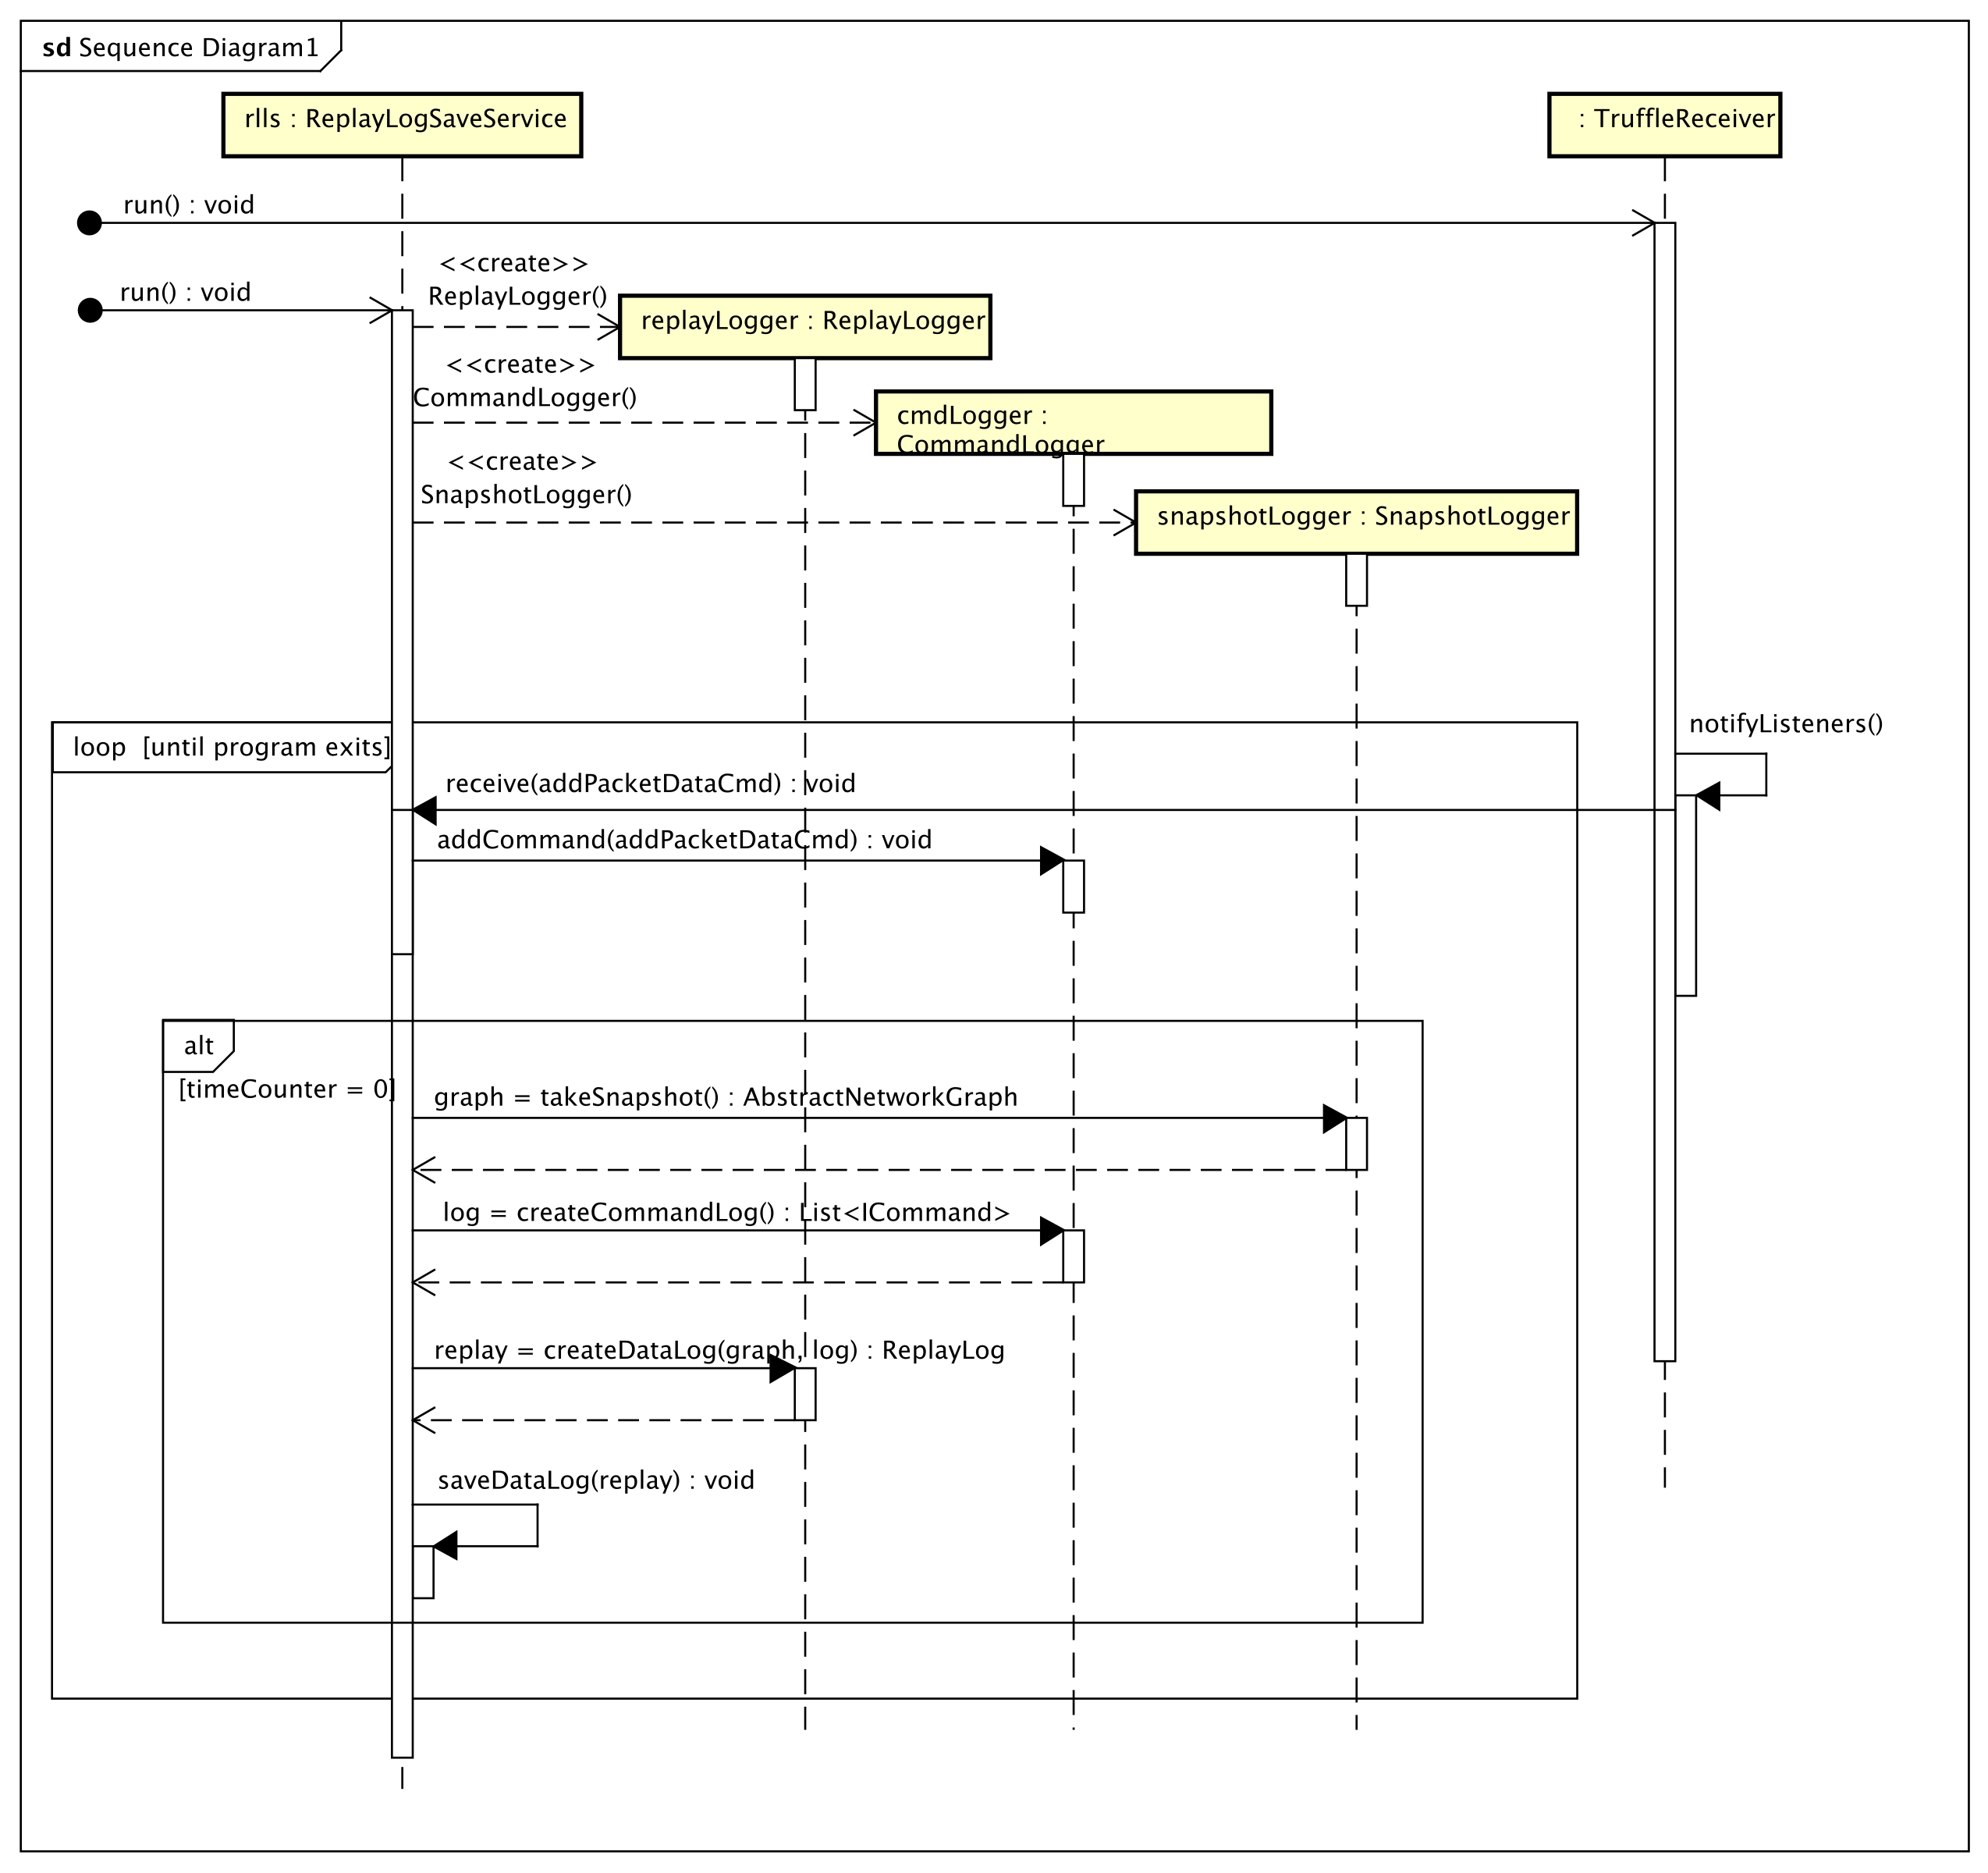
\includegraphics[width=\textwidth]{../diagramimages/sd_createsnapshot.png}
  \caption[Sequenzdiagramm DIAGRAMM]{Sequenzdiagramm DIAGRAMM}
\end{figure}

In diesem Diagramm wird die Ausführung des LoadSnapshotCommand dargestellt. Der Command wird von der View erstellt, falls der Benutzer versucht Replays anzusehen. Der Command ruft load() in dem ReplayLogLoadService auf. Dieser nimmt das übergebene Instant an und deserialisiert damit den ReplayLog. Dieser liefert den Graphen und die Commands. Im Proxy, der für den Replaygraph zuständig ist, wird der geladene Graph referenziert. Danach wird im ReplayLogLoadService das play-Flag gesetzt (da Service im eigenen Thread läuft, was zwecks besserer Übersicht ausgelassen wurde) und im NetworkGraphSwitch wird der aktuell dargestellte Graphen auf den Replaygraph umgestellt.
\subsection{DIAGRAMM}
\begin{figure}[H]
  \centering
  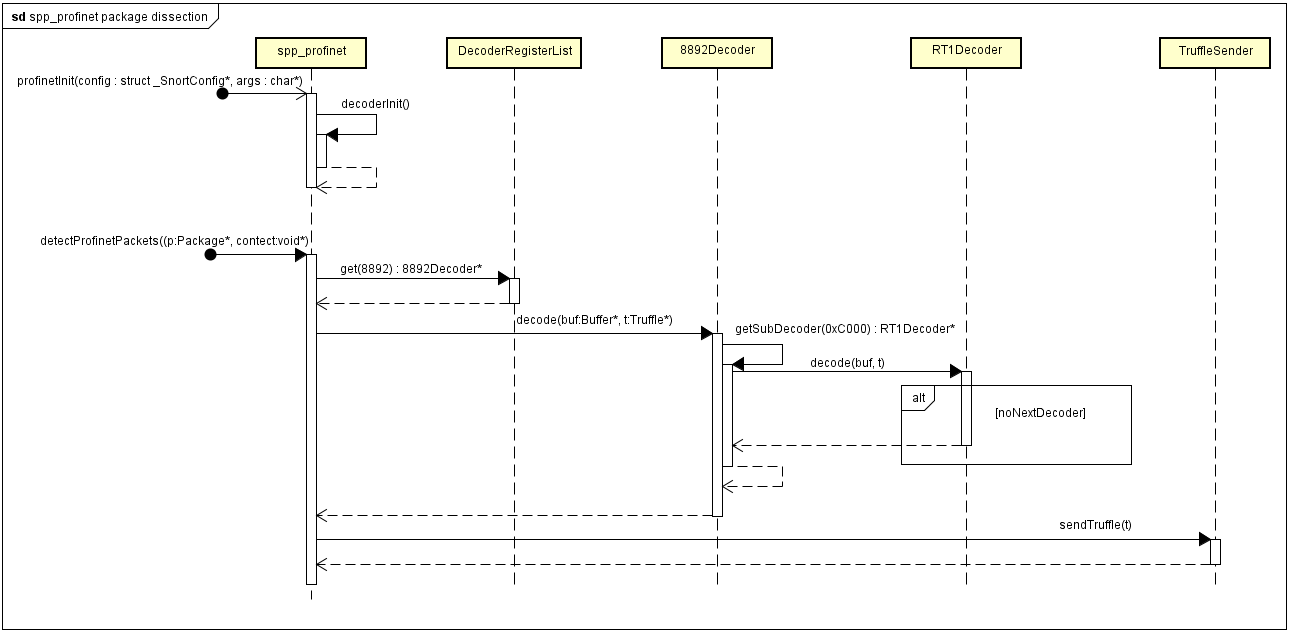
\includegraphics[width=\textwidth]{../diagramimages/spp-profinet-package-dissection.png}
  \caption[Sequenzdiagramm DIAGRAMM]{Sequenzdiagramm DIAGRAMM}
\end{figure}

 Das obige Diagramm zeigt die Speicherroutine der Commands und Snapshots des Graphen. Beim Start des ReplayLogSaveService erstellt sich dieser einen Replay-, Command- und Snapshotlogger, um sich später einen ReplayLog zusammenzustellen. Der ReplayLogSaveService ist ein Listener beim TruffleReceiver. Dadurch können die eingehenden Commands im CommandLogger gespeichert werden. Jeweils nach einem bestimmten Zeitintervall in der Endlosschleife wird ein Snapshot von dem Graphen erstellt und zusammen mit den gesammelten Commands in einem ReplayLog serialisiert.